\documentclass[12pt,a4paper]{article}
\usepackage{Setup/myStyle}
\begin{document}
\rhead{10/09/2021}						%sideopsætning
\lhead{Assignment 0}					%sideopsætning
\chead{BDSA}							%sideopsætning
\fancyfoot[C]{rkri@itu.dk}						%sideopsætning
\fancyfoot[R]{\thepage /\pageref{LastPage}}		%side x af y
\fancyfoot[L]{Rasmus Ulrik Kristensen}

%%%%%%%%%%%%%%%%%%%%%%%%%%
\begin{center}
	{\scshape\Large\bfseries \textcolor{black}{Exercise 9}\par}
	\vspace{1pt} {\large \textbf{IsLeapYear algorithm}\par}
\end{center}
\justifying

\subsubsection*{Leap year algorithm explained}
Figure \ref{fig:FlowLeapYear} shows a flowchart of the algorithm. It starts with the user input and then goes through a maximum of three if statements to test whether or not it is a leap year. It starts by evaluating if the input is lower than 1582 because then it is not a leap year and it returns false. If it is greater then it might be a leap year and it continues to evaluate if it is divisible by 100 and 400. If yes then it is a leap year and it returns true. If not then it can still be a leap year of it is divisible by 4 and not 100 and will then return true otherwise false and the algorithm is done.

\begin{figure}[H]
    \centering
    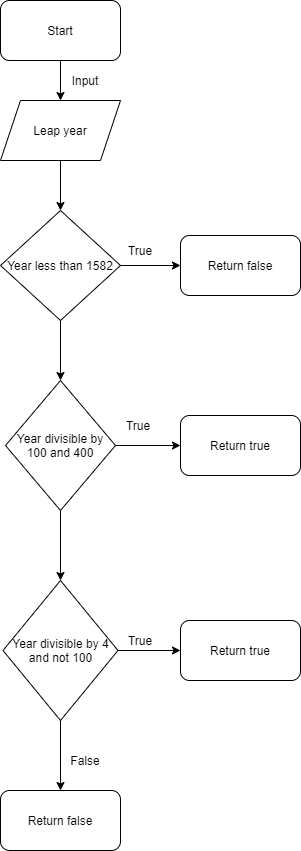
\includegraphics[height=15cm]{Exercise 8.png}
    \caption{Flowchart of IsLeapYear algorithm}
    \label{fig:FlowLeapYear}
\end{figure}



%%%%%%%%%%%%%%%%%%%%%%%%%%
\end{document}
